\documentclass[11pt,letterpaper]{report}
\usepackage[latin1]{inputenc}
\usepackage{amsmath}
\usepackage{amsfonts}
\usepackage{amssymb}
\usepackage{graphicx}
\usepackage{color}
\usepackage{enumitem}
\usepackage[dvipsnames]{xcolor}
\definecolor{codegray}{gray}{0.9}
\newcommand{\code}[1]{\colorbox{codegray}{\texttt{#1}}}
\graphicspath{{./images/}{IR}}
%\newcommand{\LF}{}  % turn on to display large format
\ifdefined \LF
\usepackage[left=2.0cm, top=2.0cm, landscape]{geometry}  % for large format landscape
\else
\usepackage[left=2.0cm, top=2.0cm]{geometry}
\fi
\usepackage{fancyhdr}
\pagestyle{fancy}
\fancyhead{}
\lhead{CS333}
\chead{Project 3 Test Report}
\rhead{Alexander DuPree}
\begin{document}
\title{Project 3 Test Report}
\author{Alexander DuPree}

\ifdefined \LF
{\Large     % large print start
\fi

  \maketitle
  \section*{Introduction}
  \noindent
  The following test report documents the tests performed for project three. The test cases and strategies closely follow the project three rubric. 

  Each section contains test cases related to the sections topic. Each test case will describe the name of the test, 
  the expected result, actual result, as well as a discussion and indication of the Pass/Fail status. 
  The actual result will be provided in the form of a screen shot of the console. 

  \section*{Compilation}
  This section presents all tests related to compiling the xv6 kernel.
  Test cases follow closely those outlined in the rubric. \hfill \break
  
  \noindent\textbf{Test Case:} \emph{With CS333\_PROJECT set to 0 in the Makefile}
  
  \noindent\textbf{Assertions:}
  \begin{enumerate}[]
  \item Code correctly compiles
  \item Kernel successfully boots
  \item \code{usertests} run to completion with all tests passed
  \end{enumerate}  
  
  \noindent\textbf{Status:} \textcolor{ForestGreen}{\textbf{PASS}}
  
  \begin{figure}[h!]
	\centering
	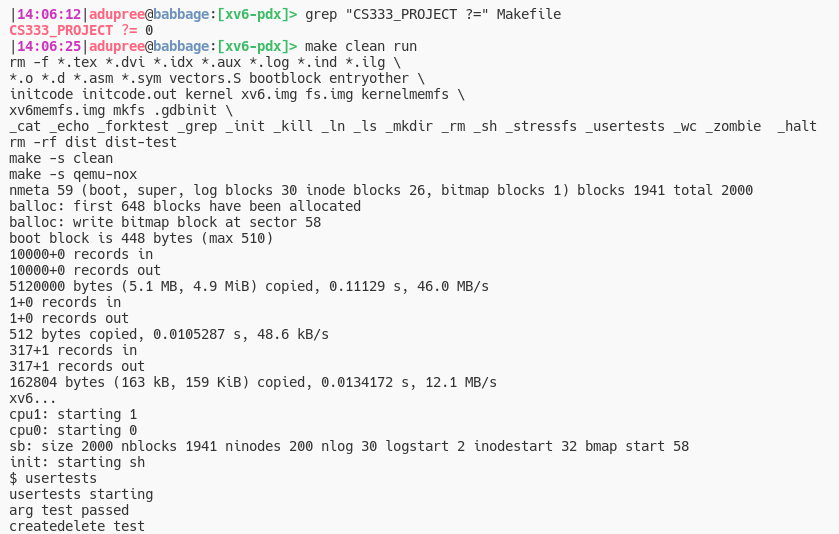
\includegraphics[width=1\linewidth]{compilation1-usertests1.png}
	\caption[img]{Compilation and boot with CS333\_PROJECT set to 0 and execution of \code{usertests}}
	\label{fig:P1compileP0-1}
  \end{figure}

  \begin{figure}[h!]
	\centering
	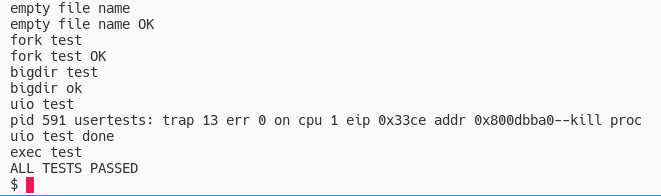
\includegraphics[width=1\linewidth]{compilation1-usertests2.png}
	\caption[img]{Completion of \code{usertests} with output elided}
	\label{fig:P1compileP0-1}
  \end{figure}

  The command \code{grep "CS333\_PROJECT ?=" Makefile} shows that the CS333\_PROJECT macro is set to 0.
  The following command \code{make clean run} demonstrates that the code correctly compiles and the kernel successfully boots. 
  Furthermore, the commands were executed within seconds of each other, indicating that
  tampering is not a possibility. Lastly, we can see that the execution of \code{usertests}
  is initiated in the same session, and Figure 2 shows that the tests run to completion and 
  all tests pass. \\

  \noindent\textbf{Test Case:} \emph{With CS333\_PROJECT set to 3 in the Makefile}
  
  \noindent\textbf{Assertions:}
  \begin{enumerate}[]
  \item Code correctly compiles
  \item Kernel successfully boots
  \item \code{usertests} run to completion with all tests passed
  \end{enumerate}  
  
  \noindent\textbf{Status:} \textcolor{ForestGreen}{\textbf{PASS}}
  
  \begin{figure}[h!]
	\centering
	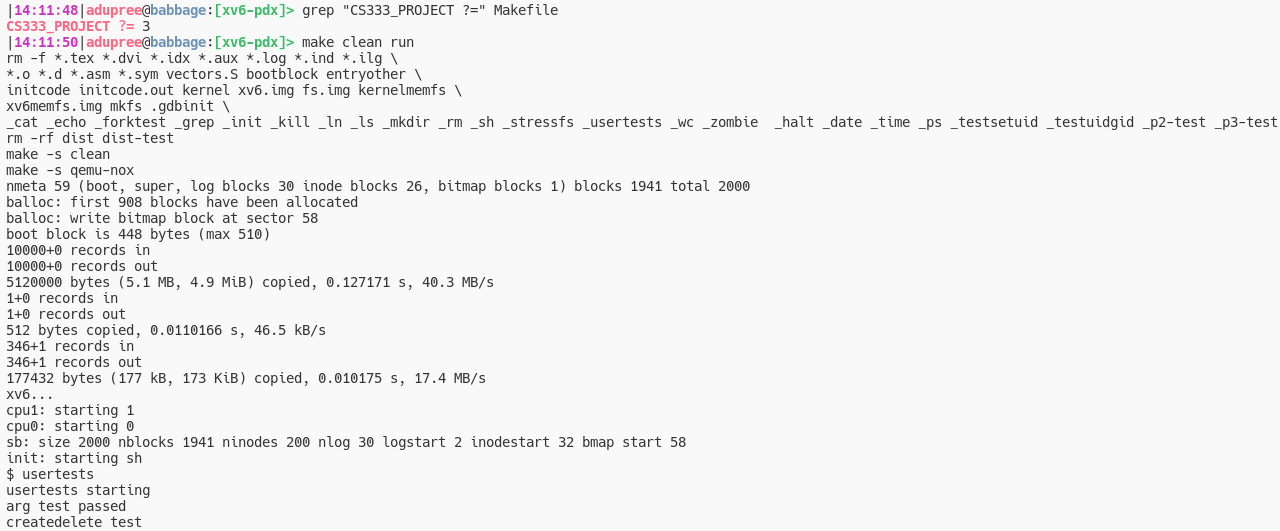
\includegraphics[width=1\linewidth]{compilation2-usertests1.png}
	\caption[img]{Compilation and boot with CS333\_PROJECT set to 3 and execution of \code{usertests}.}
	\label{fig:P1compileP0-1}
  \end{figure}

  \begin{figure}[h!]
	\centering
	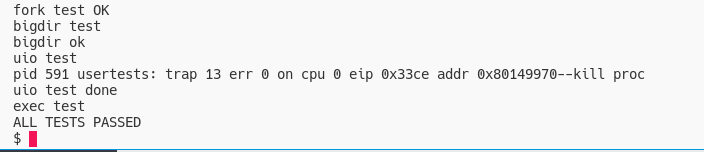
\includegraphics[width=1\linewidth]{compilation2-usertests2.png}
	\caption[img]{Completion of \code{usertests} with output elided, CS333\_P3 is defined}
	\label{fig:P1compileP0-1}
  \end{figure}

  The command \code{grep "CS333\_PROJECT ?=" Makefile} shows that the CS333\_PROJECT macro
  is indeed set to 3. The following command \code{make clean run} demonstrates that the code
  correctly compiles and the kernel successfully boots. Furthermore, the commands were executed
  within seconds of each other, indicating that tampering is not a possibility. Lastly, we can
  see that the execution of \code{usertests} is initiated in the same session and Figure 4
  demonstrates that the tests run to completion and all tests pass. \\

  \pagebreak

  \section*{State Lists and Console Commands}
  This section presents all tests related to the initilization, use, and maintenance
  of the kernels process state lists and debug console commands. 
  Test cases follow closely those outlined in the rubric. \hfill \break
  
  \noindent\textbf{Test Case:} \emph{Initialization of \code{UNUSED} list and CTRL+F console interrupt}
  
  \noindent\textbf{Assertions:}
  \begin{enumerate}[]
  \item \code{UNUSED} list is correctly initialized after XV6 boots
  \item \code{UNUSED} list is correctly updated when a process is allocated and deallocated
  \item CTRL+F correctly shows the number of \code{UNUSED} processes.
  \end{enumerate}  
  
  \noindent\textbf{Status:} \textcolor{ForestGreen}{\textbf{PASS}}
  
  \begin{figure}[h!]
	\centering
	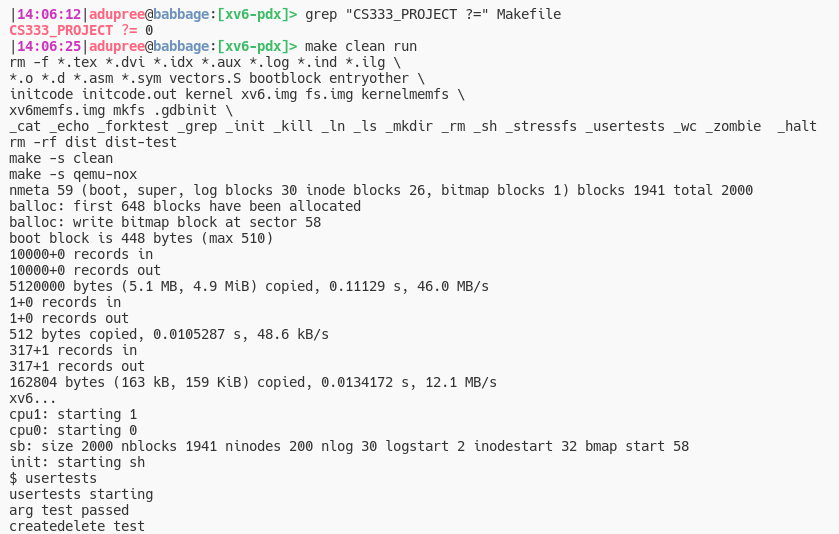
\includegraphics[width=1\linewidth]{compilation1-usertests1.png}
	\caption[img]{Compilation and boot with CS333\_PROJECT set to 0 and execution of \code{usertests}}
	\label{fig:P1compileP0-1}
  \end{figure}

  The command \code{grep "CS333\_PROJECT ?=" Makefile} shows that the CS333\_PROJECT macro is set to 0.
  The following command \code{make clean run} demonstrates that the code correctly compiles and the kernel successfully boots. 
  Furthermore, the commands were executed within seconds of each other, indicating that
  tampering is not a possibility. Lastly, we can see that the execution of \code{usertests}
  is initiated in the same session, and Figure 2 shows that the tests run to completion and 
  all tests pass. \\

\ifdefined \LF
} % large print end
\fi

\end{document}